\chapter{\label{ax:d-sustainability_and_longevity_of_nimes}Case Study. Sustainability and longevity of New Interface of Musical Expression (NIME)}

This case study aims to apply and examine the MDC model and the CATTA reactivation workflow. The MDC model can help document and archive different phases of research and versions of research outputs, while the CATTA process can be used to “reactivate” research projects that have been paused or left unfinished but still have development potential.\\
This case study's specific research field is Human-Computer Interaction (HCI) design for performances and installations, as well as for other functions, such as education and inclusion. We mainly refer to Digital Musical Instruments (DMIs) in the field of New Interfaces for Musical Expression (NIMEs).\\
The concept of New Interfaces for Musical Expression (NIME) was established around an annual conference that started as a workshop at CHI 2001. Over its twenty-three years, NIME has become a leading event in music technology, emphasising design and human-computer interaction (HCI) for performances and installations. It covers various topics—from Digital Musical Instrument (DMI) design, technology, and protocols to education, generative music, and machine learning—highlighting its interdisciplinary nature involving engineers, scientists, and artists \cite{fasciani202120}.\\
A significant challenge in the context of NIME is the longevity of the research outcomes. Many new DMIs are introduced at the conference each year, yet few remain in use beyond one performance \cite{mamedes2014nime, morreale2017nime}. Accelerated technological trends \cite{devine2019decomposed, burkart2012cyberliberties} and an academic environment that values innovation over long-term use \cite{marquez2015fourteenyears, heyes2020nime} contribute to this issue. Recent reviews indicate that although the NIME community is increasingly concerned about reuse and documentation, most of the new work still focuses on introducing new technologies \cite{masu2023nime}.\\
To address this issue, the MDC (Multilevel Dynamic Conservation) and CATTA process models are being explored as possible solutions for improving sustainability and reusability within NIME. The technological setup for these research projects, as well as the tools and instruments used and those created, are the same as those found in live media artworks. Therefore, while we use this research area to refine how we apply the systems introduced in this text, we also propose viewing the specific outcomes of these projects as live media art themselves, with the goal of supporting their long-term sustainability \cite{fiordelmondo2024nime}.\\
This case study includes \textit{Soundrise}, an interactive multimedia application for deaf children, and two DMIs (\textit{Electronic\_Khipu\_} and \textit{Kanchay\_Yupana//}), both documented using GitHub. The case study was conducted in collaboration with Assistant Professor Raul Masu and the Computational Media and Arts (CMA) Department at the Hong Kong University of Science and Technology (Guangzhou).

\section{Objectives}
The main objectives of this case study, in addition to applying, testing, and refining the systems introduced in Chapter~\ref{ch:3-mdc_model-reactivation_workflow-instruction_template}, are:
\begin{enumerate}
    \item exploring and studying the interdisciplinary collaboration processes and systems that support the development of live media art technologies, tools, and artworks themselves;
    \item examining conservation and reactivation in the context of international and interdisciplinary research projects;
    \item studying the technologies basis of live media artworks;
    \item developing GitHub repositories according to the MDC model—see Chapter~\ref{ch:4-madc_model_application} for more details.
\end{enumerate}

\section{Introduction}
\subsection*{Soundrise}
\textit{Soundrise} is an educational game created by the Centro di Sonologia Computazionale (CSC) in 2012 to help children, especially those who are deaf, explore and understand their voices. It consists of a basic HCI interface which uses real-time analysis of vocal features, showing a sun on the screen that changes its position, size, and colour based on the child's voice's pitch, intensity, and timbre.\\
Initially built in Pure Data (Pd) with the timbreID library, \textit{Soundrise} was later adapted to C++ and libpd to improve its usability on different platforms and enhance its graphical interface. Early usability tests confirmed the application's effectiveness, although it still needed improvement.\\
In 2023, CSC initiated new thesis projects to update \textit{Soundrise} and encourage further research on sound technologies for people with special hearing needs. These projects focused on conserving the original research while modernising the application. They developed using the same approach used for live media artworks, porting the program to a web environment, using JavaScript, Three.js, React.js, and Web Audio API for real-time audio analysis. These projects led to a complete Web app version of \textit{Soundrise}, integrating vowel recognition and a more advanced interface \cite{fiordelmondo2024nime}.
\subsection*{Patricia Cadavid's DMIs}

\begin{figure}[!h]
    \centering
    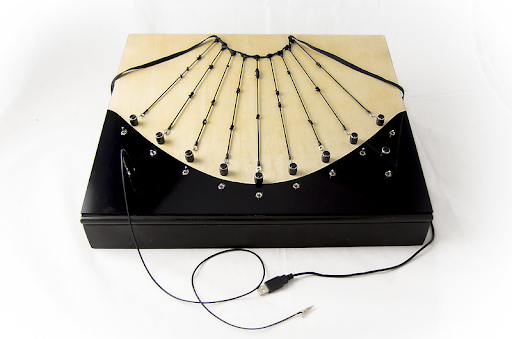
\includegraphics[width=\linewidth]{chapters/appendix/d/image/figd-khipu.png}
    \caption{The \textit{Electronic\_Khipu\_} developed by Patricia Cadavid.}
    \label{fig:ad-khipu}
\end{figure}

Patricia Cadavid is a Colombian artist and researcher based in Europe who emphasises her identity as an immigrant. Her artistic work focuses on the relationships and effects of colonialism in new media, drawing from her experiences with migration and adopting decolonial and anti-colonial perspectives. She focuses on developing New Interfaces for Musical Expression (NIMEs) for audiovisual performances. Over the past four years, she has created two main digital musical instruments (DMIs): the \textit{Electronic\_Khipu\_} and the \textit{Kanchay\_Yupana//}, both inspired by pre-colonial Andean technologies.\\
The \textit{Electronic\_Khipu\_} (see Figure~\ref{fig:ad-khipu}) is a NIME designed to create live experimental sounds through knot-making with conductive rubber cords. It is inspired by the \textit{Khipu}, an ancient Incan device for storing and transmitting information. The \textit{Electronic\_Khipu\_} aims to revive this ancient device with a new interpretation. Instead of viewing it solely as a numerical system, the \textit{Electronic\_Khipu\_} uses the \textit{Khipu}’s code system to create new messages and sound stories. Patricia introduced the \textit{Electronic\_Khipu\_} at NIME 2020, presenting a paper and a performance titled \textit{Knotting the Memory//Encoding the Khipu\_} \cite{cadavid2020knotting, hinojosa2020electronic_khipu_, cadavid2022knotting}.\\
The \textit{Kanchay\_Yupana//} is another NIME created to generate musical rhythms (see Figure~\ref{fig:ad-yupana}). Inspired by the \textit{Yupana}, an Andean device similar to an abacus used for arithmetic calculations, the \textit{Kanchay\_Yupana//} complements the \textit{Electronic\_Khipu\_} by creating patterns that transform into rhythms and sounds during live performances. Patricia introduced the \textit{Kanchay\_Yupana//} at NIME 2022 and presented it with the performance \textit{Regreso a la Tierra} at the Cultural Center of Spain in Santiago, Chile \cite{hinojosa2022kanchay_yupana, cadavid2022knotting}.\\

\begin{figure}[!h]
    \centering
    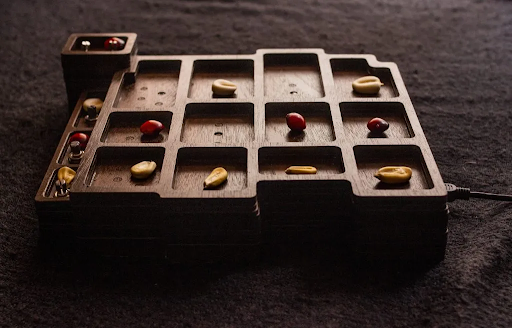
\includegraphics[width=\linewidth]{chapters/appendix/d/image/figd-yupana.png}
    \caption{The \textit{Kanchay\_Yupana//} developed by Patricia Cadavid.}
    \label{fig:ad-yupana}
\end{figure}

Patricia Cadavid’s instruments and the multimedia application \textit{Soundrise} have been archived using the MDC (Multilevel Dynamic Conservation) model on GitHub as public repositories\footnote{The GitHub repositories can be found at the link (\textit{Electronic\_Khipu\_}) \url{https://github.com/alessandrofiordelmondo/cadavid_khipu}, (\textit{Kanchay\_Yupana//}) \url{https://github.com/alessandrofiordelmondo/cadavid_yupana}}. This archiving with public repositories ensures the longevity of these NIMEs by making them easy to share, update, and replicate. For more details on using the MDC model in a GitHub repository see Chapter~\ref{ch:4-madc_model_application}. In the following sections, we will discuss the reactivation of \textit{Soundrise} and the compilation of its score.

\section{Reactivation}
While Cadavid's instruments have only been documented and archived to enable future replications, the \textit{Soundrise} application has been reactivated through multiple efforts. These efforts especially include Giada Zuccolo's thesis \cite{zuccolo2023soundrise} and the NIME paper \cite{fiordelmondo2024nime}, which contributed to formalising the CATTA process. The steps for reactivation are summarised below, for further details refer to the NIME paper \cite{fiordelmondo2024nime}.\\

\subsection*{Collection}
The first step was to gather the initial versions of the \textit{Soundrise} application for analysis during its reactivation. We created three main \textit{Iteration Folder}s (IFs) representing three versions of the app, each linked to two master’s theses \cite{randon2012soundrise, giusto2012soundrise} and one bachelor’s thesis \cite{turetta2023soundrise}. These theses provided detailed information and experiences, including design details, evaluations, descriptions of DSP algorithms, and mappings for audio-to-visual interactions. Additionally, we accessed the applications and source codes developed in Pure Data, C++, and JavaScript, stored on CSC server We organised all these materials using the MDC model to show how \textit{Soundrise} evolved across different versions.

\subsection*{Assessment}
We reviewed all the collected materials to identify problems and strengths in the previous versions of \textit{Soundrise}. The older versions had several issues. The Pure Data (PD) version \cite{giusto2012soundrise} required installing the software and learning settings, making it difficult for children to use. It was also not compatible with mobile devices, which many children use instead of computers. The C++ \cite{randon2012soundrise} version needed constant updates for different operating systems and libraries. Its interface used OpenGL, which is outdated and not maintained, limiting the app’s long-term preservation. JavaScript version \cite{turetta2023soundrise}, although it could solve some problems, it only handled the graphics part and relied on external software for creating the user interface (Blender), making it incomplete for future improvements.\\
On the contrary, based on the three theses and a demo video, we found potential in previous versions. We learned that the app’s simple graphic design helped children understand the visual feedback.\\
Based on this assessment, we defined the \textit{Design space}, focusing on making the app long-lasting and easy to maintain by choosing web-based technology. Web apps can be used on any device with a browser, are scalable, and can easily connect with other web services. Using web-based libraries also helps prevent the app from becoming outdated.\\
We selected a series of development paths considering longevity, future improvements, and updates. We analysed trends in usability and popularity of tools for web development. We selected ReactJS as the development environment’s front-end framework since it reports the greatest popularity, as shown by the 2022 \textit{State of JS} and the \textit{Stack Overflow Trends service}.

\subsection*{Transcription}
The first step of the transcription involved the Digital Signal Processing algorithms. We decided to move away from using Pure Data (PD) objects and instead take advantage of the browser’s audio capabilities by using the Web Audio API—a high-level JavaScript tool that allows sound processing within a web application.\\
The main algorithms we developed with the Web Audio API, based on the older versions, are \textit{audio intensity detection} (implemented using an RMS algorithm similar to the old versions), \textit{voice pitch detection} (switched from an FFT-based method in PD to an auto-correlation algorithm) and \textit{vowel extraction}. We explored different development paths for the \textit{vowel extraction} algorithm, created prototypes, and conducted evaluations. We considered porting the original PD and timbreID to the Web Audio API, using \textit{APEWORM} (an existing real-time vowel detection tool for the web that hasn’t been updated since 2017), and creating a new system. The third option proved to be the most effective, so we developed our own vowel detection using the Web Audio API based on \textit{Linear Predictive Coding} (LPC) and formant extraction. This method avoids using external libraries, making it easier to maintain.\\
The second step was developing the interface, which also involved exploring different approaches and considering whether or not to use external tools like Blender and Three.js. To make future updates easier, we decided not to use external software. Instead, we built the interface entirely with ReactJS and CSS animations. This kept the design simple and ensured that the voice feedback was easy for users to understand.\\
By making these choices, we simplified the application’s design and improved its compatibility and maintainability.

\subsection*{Transmission}
After studying all development paths within the defined design space and producing several prototypes, we finally achieved an efficient and functioning front-end application that relies almost exclusively upon ReactJS. In the transmission phase, we focused on distributing the web application. We used the web hosting service provided by Firebase for the application deployment. To promote future improvements and developments of the application and related research, we licensed the web application with the open-source GNU \textit{General Public License v3.}0 (GPLv3.0).

\subsection*{Archiving}
All the documentation produced in the previous steps of the reactivation process has been archived as a GitHub repository according to the MDC model. We added a fourth IF, a new iteration of the \textit{Soundrise} application (Figure~\ref{fig:ad-graph-mdc}).
Details on the application of the MDC model on GitHub can be found in Chapter~\ref{ch:4-madc_model_application}\footnote{{The \textit{Soundrise} GitHub repository's can be found at the link \url{https://github.com/CSCPadova/soundrise-prj/tree/main}}}.

\section{Data compilation}
We report some \textit{Soundrise} application mappings based on the data compilation through MIF and BVL systems introduced in Chapter~\ref{ch:3-mdc_model-reactivation_workflow-instruction_template} and \ref{ch:4-madc_model_application}. Since we are dealing with a web application, we don’t have spatial mapping or other instructions in this case. Also, the \textit{bit} list is small since we just need a phone with a browser at the implementation level. Nevertheless, we report the conceptual, physical implementation, and process mappings.

\subsection*{Conceptual mapping}
For the \textit{conceptual mapping}, we can develop two specification levels, from a general overview of the application to a specific one, highlighting the role of each of the voice’s features. Figure~\ref{fig:ad-mapping-conceptual} shows the relationship between the voice and the movement of the sound; Figure~\ref{fig:ad-mapping-conceptual02} shows the relationship between the intensity, pitch, and vowels produced by the voice with the vertical, size, and colour transformation of the sun on the screen.

\begin{figure}[!h]
    \centering
    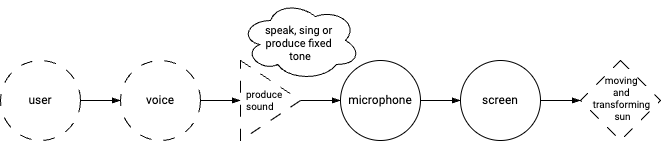
\includegraphics[width=\linewidth]{chapters/appendix/d/image/graphd-mapping-conceptual.drawio.png}
    \caption{\textit{Conceptual mapping} at the highest level of representation}
    \label{fig:ad-mapping-conceptual}
\end{figure}

\begin{figure}[!h]
    \centering
    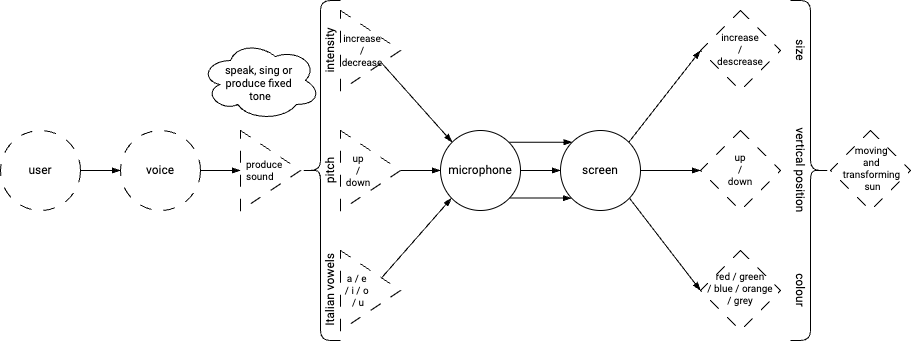
\includegraphics[width=\linewidth]{chapters/appendix/d/image/graphd-mapping-conceptual02.drawio.png}
    \caption{\textit{Conceptual mapping} at a lower level of representation, with the description of the relationship between the audio features and the sun movements. }
    \label{fig:ad-mapping-conceptual02}
\end{figure}

\subsection*{Physical implementation mapping}
Since we have a minimal \textit{bit} list, the \textit{physical implementation mapping} will also be very tight. Figure~\ref{fig:ad-mapping-physical} shows the physical implementation considering only the smartphone microphone, screen, and application (the browser). 

\begin{figure}[!h]
    \centering
    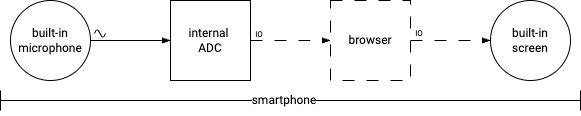
\includegraphics[width=\linewidth]{chapters/appendix/d/image/graphd-mapping-physical.png}
    \caption{\textit{Physical implementation mapping} of \textit{Soundrise} application.}
    \label{fig:ad-mapping-physical}
\end{figure}

\subsection*{Process mapping}
Figure~\ref{fig:ad-mapping-process} shows \textit{Soundrise}’s process mapping at the highest level. It includes all the specific functions, such as the \textit{rms}, \textit{pitchAutcorrel}, \textit{downsampling}, etc. which can be further represented with other mappings describing the process at a lower level. Figure~\ref{fig:ad-mapping-process02} show an example of the \textit{rms} function.

\begin{figure}[!h]
    \centering
    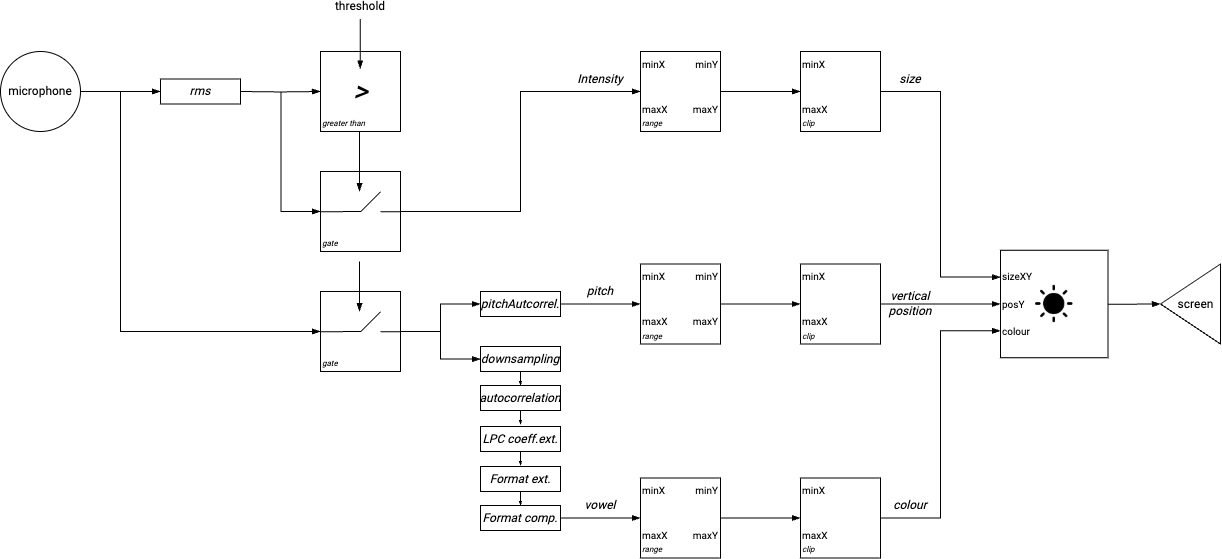
\includegraphics[width=\linewidth]{chapters/appendix/d/image/graphd-mapping-process.png}
    \caption{\textit{Soundrise}’s \textit{Process mappings} at the highest level.}
    \label{fig:ad-mapping-process}
\end{figure}

\begin{figure}[!h]
    \centering
    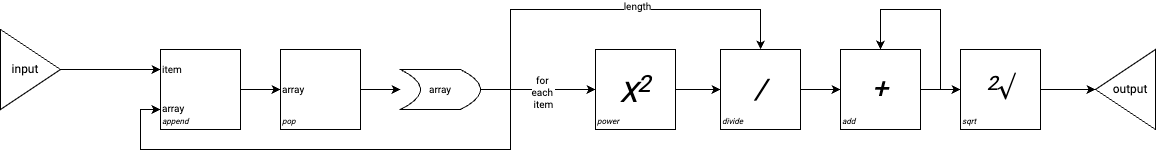
\includegraphics[width=\linewidth]{chapters/appendix/d/image/graphd-mapping-process02.drawio.png}
    \caption{\textit{Soundrise}’s \textit{Process mappings} of the \textit{rms} function.}
    \label{fig:ad-mapping-process02}
\end{figure}

\section{Results and discussion}
Though not focused on artworks (thus omitting some key aspects of the main project's focus), these case studies still present challenges of obsolescence, technology migration and adaptation, interactivity, documentation, and archiving that are close to those encountered in live media art. The studies are particularly valuable from a practical perspective, as they are research projects—one in the educational and inclusive field (\textit{Soundrise}) and the other (Patricia Cadavid’s instruments) of Design, HCI, and the arts.\\
Beyond the technological and archiving issues, these studies present other interesting characteristics. They are in an ongoing development phase (meaning they are not ``finished'' and ``fixed'') and are evolving in broad interdisciplinary and collaborative contexts. For example, Cadavid’s instruments involve a collaboration across China, Europe, and South America, including artists, humanists, computer scientists, and designers.\\
The specific requirements of these research projects guide the application of the MDC model on the GitHub platform. GitHub allows for collaborative work on repositories, enabling simultaneous development and version tracking. As detailed in Chapter~\ref{ch:4-madc_model_application}, applying the MDC model in line with GitHub’s collaborative development paradigms has proven especially challenging.\\
Therefore, the case study has produced positive results within the project’s main area of focus, as well as in the context of NIME research. On one hand, these studies led to the formalisation of the CATTA reactivation workflow and the modelling of the MDC model within the GitHub platform, thus contributing to the development and collaboration platforms that could potentially be used for archiving artworks. On the other hand, the model proved effective within the NIME research field, contributing a new approach for the documentation and archiving of research outcomes, and therefore to the longevity and sustainability of NIMEs \cite{fiordelmondo2024nime}.

\begin{figure}[!h]
    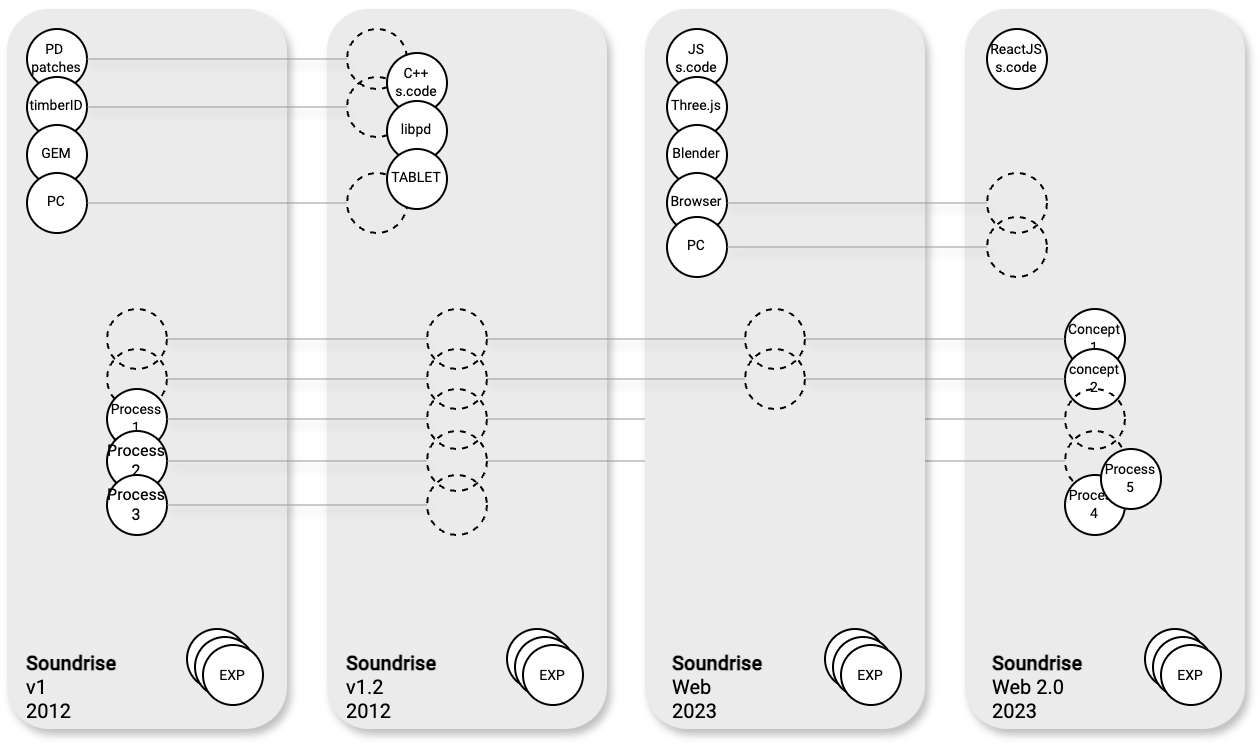
\includegraphics[width=\linewidth]{chapters/appendix/d/image/graphd-mdc.png}
    \caption{The four iterations of \textit{Soundrise} archived according to the MDC model.}
    \label{fig:ad-graph_mdc}
\end{figure}














